\documentclass[authoryear,preprint]{sigplanconf}
\usepackage{amsmath}
\usepackage{listings} 
\usepackage{stmaryrd}
\usepackage{latexsym}
\usepackage{amssymb}
\usepackage{xcolor}
\usepackage{courier}
\usepackage{thmtools}
\usepackage{bbold}
\usepackage{tikz}

\newcommand{\lolli}{\multimap} 
\newcommand{\cubt}{\mathbb{T}}
\newcommand{\den}[1]{\llbracket #1 \rrbracket}
\newcommand{\denc}[1]{\llbracket #1 \rrbracket^c}
\newcommand{\nodet}[2]{\fcolorbox{black}{white}{$#1$}\fcolorbox{black}{gray!20}{$#2$}}

\begin{document}
\special{papersize=8.5in,11in}
\setlength{\pdfpageheight}{\paperheight}
\setlength{\pdfpagewidth}{\paperwidth}

\newcommand{\alt}{~|~}
\lstnewenvironment{code}{\lstset{basicstyle={\sffamily\footnotesize}}}{}

\lstset{frame=none,
         language=Haskell,
         basicstyle=\sffamily, 
         numberstyle=\tiny,
         numbersep=5pt,
         tabsize=2,    
         extendedchars=true,
         breaklines=true,   
         breakautoindent=true,
         keywordstyle=\color{black},
         captionpos=b,
         stringstyle=\color{black}\ttfamily,
         showspaces=false,  
         showtabs=false,    
         framexleftmargin=2em,
         framexbottommargin=1ex,
         showstringspaces=false
         basicstyle=\sffamily,
         columns=[l]flexible,
         flexiblecolumns=true,
         aboveskip=\smallskipamount,
         belowskip=\smallskipamount,
         lineskip=-1pt,
         xleftmargin=1em,
         escapeinside={/+}{+/},
         keywords=[1]{Monad,Just,Nothing,type,data,right,left,id,where,do,
                     if,then,else,let,in},
         literate=
           {+}{{$\;+\;$}}1 
           {/}{{$/$}}1 
           {*}{{$\;*\;$}}1
           {=}{{$=\ $}}1 
           {/=}{{$\not=$}}1
           {[]}{$[\;]$}2
           {<}{{$<$}}1 
           {>}{{$>$}}1 
           {++}{{$+\!\!\!+\;$}}1 
           {::}{{$:\mkern -2.5mu:\;$}}1
           {&&}{{$\&\!\!\!\&$}}2
           {:=:}{{$:\mkern -2mu=\mkern -2mu:\;$}}3
           {:+:}{{$:\mkern -5mu+\mkern -5mu:\;$}}3
           {:-:}{{$:\mkern -5mu-\mkern -5mu:\;$}}3
           {:*:}{{$:\mkern -5mu*\mkern -5mu:\;$}}3
           {$}{{\texttt{\$}\hspace{0.5em}}}1
           {`}{$^\backprime$}1
           {==}{{$=\!=\;$}}2
           {===}{{$\equiv\;$}}2
           {->}{{$\rightarrow\;$}}2 
           {>=}{{$\geq$}}2 
           {<=}{{$\leq$}}2 
           {>=0}{{$\geq_\zerog\;$}}2 
           {<=0}{{$\leq_\zerog\;$}}2 
           {==0}{{$=_\zerog\;$}}2 
           {>0}{{$>_\zerog\;$}}2 
           {<0}{{$<_\zerog\;$}}2 
           {<-}{{$\leftarrow$}}2
           {=>}{{$\Rightarrow\;$}}2
           {<<}{{$\ll$}}2 
           {>>}{{$\gg\;$}}2
           {>>>}{{$\ggg\;$}}3 
           {<<<}{{$\lll\;$}}3
           {>>=}{{$\gg\mkern -2.5mu=\;$}}3
           {=<<}{{$=\mkern -2.5mu\ll\;$}}3
           {<|}{$\lhd\;$}2
           {<||}{$\unlhd\;$}2
           {\ ||\ }{$\|$}1
           {\\}{$\lambda$}1
           {:>}{{$\rhd$}}2
           {||>}{{$\unrhd$}}2
           {_}{{$\_$}}1
           {_B}{{$_b$}}2
           {forall}{{$\forall$}}1
}

\lstset{postbreak=\raisebox{0ex}[0ex][0ex]
        {\ensuremath{\hookrightarrow}}}
\lstset{breaklines=true, breakatwhitespace=true}
\lstset{numbers=none, numbersep=5pt, stepnumber=2, numberstyle=\scriptsize}
\lstset{rangeprefix=/*!\ , rangesuffix=\ !*\/, includerangemarker=false}

%% double-blind reviewing...
\title{Cubical Types with Positive and Negative Polarities}
\authorinfo{}{}{}
\maketitle

\begin{abstract}
\ldots
\end{abstract}

%%%%%%%%%%%%%%%%%%%%%%%%%%%%%%%%%%%%%%%%%%%%%%%%%%%%%%%%%%%%%%%%%%%%%%%%%%%%%%
\section{Introduction}

The \textbf{Int} construction or the $\mathcal{G}$ construction are neat. As
Neel K. explains, given first-order types and feedback you get higher-order
functions. But if you do the construction on the additive structure, you lose
the multiplicative structure. It turns out that this is related to a deep
open problem in algebraic topology and homotopy theory that was recently
solved. We ``translate'' that solution to a computational type-theoretic
world. This has evident connections to homotopy (type?) theory that remain to
be investigated.

%%%%%%%%%%%%%%%%%%%%%%%%%%%%%%%%%%%%%%%%%%%%%%%%%%%%%%%%%%%%%%%%%%%%%%%%%%%%%%
\section{The \textbf{Int} Construction} 

Explain in detail perhaps with Haskell embedding and type functions etc. The
key insight it to add ``negative'' types representing demand for values. This
is how you get functions.

%%%%%%%%%%%%%%%%%%%%%%%%%%%%%%%%%%%%%%%%%%%%%%%%%%%%%%%%%%%%%%%%%%%%%%%%%%%%%%
\section{The Problem and the Intuitive Solution}

We lose the multiplicative structure. No evident way to define the
multiplication functor. Perhaps there is a clever way. But this turns out to
be a well-known open problem. Review the problem and tell the story from the
algebraic topology perspective.

Regular first-order types are viewed as 1-dimensional cubes. Generalize to
$n$-dimensional cubes. 

%%%%%%%%%%%%%%%%%%%%%%%%%%%%%%%%%%%%%%%%%%%%%%%%%%%%%%%%%%%%%%%%%%%%%%%%%%%%%%
\section{The Formal Construction} 

We use $t$ for regular first-order types which include the empty type, the
unit type, and conventional sum and product types.  We use $\tau$ for cubical
types: these have the same formal structure as regular types but also include
\emph{negative} types. The syntax of the types is summarized below:
\[\begin{array}{rcl}
t &::=& 0 \alt 1 \alt t_1 + t_2 \alt t_1 * t_2 \\
\tau &::=& t \alt 
      \alt \tau_1 + \tau_2
      \alt \tau_1 * \tau_2
      \alt - \tau
\end{array}\]
We use $\tau_1 - \tau_2$ to abbreviate $\tau_1 + (- \tau_2)$ and more
interestingly $\tau_1 \lolli \tau_2$ to abbreviate $(- \tau_1) + \tau_2$. At
the level of cubical types, we can write types such as
$(t_1-t_2)-(t_3-t_4*t_5)$ which mix negative types with the usual type
constructors.

It is easy to find a model for regular types: finite sets are such a
model. In more detail:
\[\begin{array}{rcl}
\den{0} &=& \emptyset \\
\den{1} &=& \{ \bullet \} \\
\den{t_1 + t_2} &=& \den{t_1} \uplus \den{t_2} \\
\den{t_1 * t_2} &=& \den{t_1} \times \den{t_2} 
\end{array}\]
The type 0 maps to the empty set. The type 1 maps to a singleton set. The sum
of types maps to disjoint union of sets. The product of types maps to the
cartesian product of sets. We usually use $S$ for the denotation of a
conventional first-order type.

For cubical types, their denotations, usually written as $\cubt$, are
$n$-dimensional cubical sets with polarities. An $n$-dimensional cubical set
$\nodet{\cubt_1}{\cubt_2}$ consists of a positive subspace $\cubt_1$ and a
negative subspace $\cubt_2$ (shaded in gray). Each of the subspaces are
cubical set of a lower dimension; the 1-dimensional case reduces to
$\nodet{S}{\phantom{S}}$ which is essentially the denotation of
conventional first-order types. As we explain below, cubical sets are closed
under sums, differences, products.

Examples of 1-dimensional cubical sets include all the sets of the form
$\nodet{S}{\phantom{S}}$ where $S$ is finite set denoting a regular
first-order types $t$. A 2-dimensional cubical set looks like
$\nodet{S_1}{S_2}$ which intuitively corresponds to the difference $t_1 -
t_2$ of the two types whose denotations are $S_1$ and $S_2$ respectively. A
3-dimensional cubical type looks like
$\nodet{(\nodet{S_1}{S_2})}{(\nodet{S_3}{S_4})}$ which intuitively
corresponds to the iterated difference of the appropriate types
$(t_1-t_2)-(t_3-t_4)$ where the successive colors from the root encode the
sign as follows: white in the outermost box corresponds to a positive
polarity and gray in the outermost box corresponds to a negative polarity;
then, as we move inwards the polarities alternate for every change of color.

We now give the denotation of cubical types:
\[\begin{array}{rcl}
\denc{t} &=& \nodet{\den{t}}{\phantom{\den{t}}} = 
  \nodet{\nodet{\den{t}}{\phantom{\den{t}}}}{\phantom{\den{t}}} = \ldots \\
\\
\denc{\tau_1 + \tau_2} &=& \denc{\tau_1} \oplus \denc{\tau_2} \\
\denc{\tau_1 * \tau_2} &=& \denc{\tau_1} \otimes \denc{\tau_2} \\
\denc{- \tau} &=& \ominus \denc{\tau}
\end{array}\]
where the operations $\oplus$, $\otimes$, and $\ominus$ are defined below.
It is possible for cubical types not be balanced in general but it is always
possible to embed an $n$-dimensional set into a larger dimension using the
equivalence in the first clause which formalizes that $t$ is equivalent to
$t-0$ and to $(t-0)-0$ etc.  In the recursive definitions below, we assume
that the types have been extended to be balanced as needed:
\[\begin{array}{rcl}
\ominus~S &=& S \\
\ominus~\nodet{\cubt_1}{\cubt_2} &=& \nodet{\ominus~\cubt_2}{\ominus~\cubt_1} \\
\\
S_1 \oplus S_2 &=& S_1 \uplus S_2 \\
(\nodet{\cubt_1}{\cubt_2}) \oplus (\nodet{\cubt_3}{\cubt_4}) &=& 
  \nodet{\cubt_1 \oplus \cubt_3}{\cubt_2 \oplus \cubt_4} \\
\\
S_1 \otimes S_2 &=& S_1 \times S_2 \\
S \otimes (\nodet{\cubt_1}{\cubt_2}) &=& 
  \nodet{S \otimes \cubt_1}{S \otimes \cubt_2} \\
(\nodet{\cubt_1}{\cubt_2}) \otimes \cubt &=& 
  \nodet{\cubt_1 \otimes \cubt}{\cubt_2 \otimes \cubt}
\end{array}\]

\begin{figure*}
\[\begin{array}{c}
\nodet{S_1}{S_2}
\quad\otimes\quad
\nodet{(\nodet{S_3}{S_4})}{(\nodet{S_5}{S_6})} = 
\\
\nodet{(\nodet{{(\nodet{S_1 \times S_3}{S_1 \times S_4})}}
              {{(\nodet{S_1 \times S_5}{S_1 \times S_6})}})}
      {(\nodet{{(\nodet{S_2 \times S_3}{S_2 \times S_4})}}
              {{(\nodet{S_2 \times S_5}{S_2 \times S_6})}})}
\end{array}\]
\caption{\label{mult}Example of multiplication of two cubical types.}
\end{figure*}

The definition of negation is natural: it recursively swaps the positive and
negative subspaces. We note that the general definitions of sum and product
reduce to the conventional sums and products for 1-dimensional types. Also
the sum of 2-dimensional types reduces to the sum used in the \textbf{Int}
construction. The interesting new development is the product definition. The
example in Fig.~\ref{mult} shows that in general the product of an
$n$-dimensional type with an $m$-dimensional type gives an
$(n+m)$-dimensional type. For low dimensions such as the ones used in the
example above, it is possible to visualize what is happening in coordinate
space (see Fig.~\ref{multv}).

\begin{figure*}
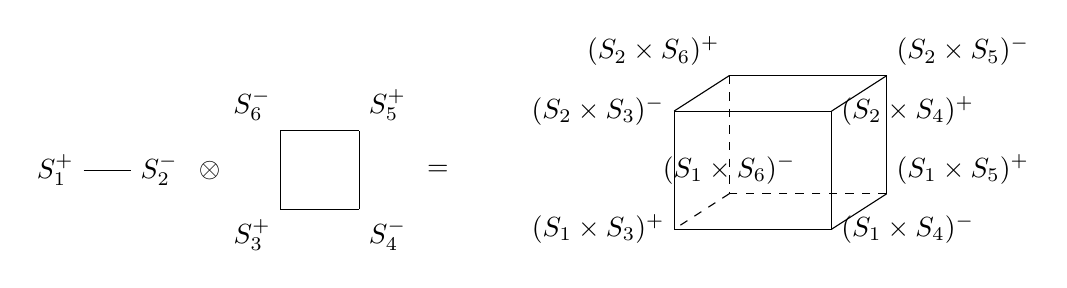
\begin{tikzpicture}
\node[left] at (0,0) {$S_1^+$};
\node[right] at (0.6,0) {$S_2^-$};
\draw[-] (0,0) -- (0.6,0);
\node at (1.6,0) {$\otimes$}; 
%%
\node[below left] at (2.5,-0.5) {$S_3^+$};
\node[below right] at (3.5,-0.5) {$S_4^-$};
\draw[-] (2.5,-0.5) -- (3.5,-0.5);
\draw[-] (2.5,-0.5) -- (2.5,0.5);
\node[above left] at (2.5,0.5) {$S_6^-$};
\node[above right] at (3.5,0.5) {$S_5^+$};
\draw[-] (2.5,0.5) -- (3.5,0.5);
\draw[-] (3.5,-0.5) -- (3.5,0.5);
%% 
\node at (4.5,0) {$=$};
%% 
\node[left] at (7.5,0.75) {$(S_2 \times S_3)^-$};
\node[right] at (9.5,0.75) {$(S_2 \times S_4)^+$};
\node[above right] at (10.2,1.2) {$(S_2 \times S_5)^-$};
\node[above left] at (8.2,1.2) {$(S_2 \times S_6)^+$};
%%
\node[left] at (7.5,-0.75) {$(S_1 \times S_3)^+$};
\node[right] at (9.5,-0.75) {$(S_1 \times S_4)^-$};
\node[above right] at (10.2,-0.3) {$(S_1 \times S_5)^+$};
\node[above] at (8.2,-0.3) {$(S_1 \times S_6)^-$};
%%
\draw[-] (7.5,0.75) -- (9.5,0.75);
\draw[-] (9.5,0.75) -- (10.2,1.2);
\draw[-] (10.2,1.2) -- (8.2,1.2);
\draw[-] (8.2,1.2) -- (7.5,0.75);
%%
\draw[-] (7.5,-0.75) -- (9.5,-0.75);
\draw[-] (9.5,-0.75) -- (10.2,-0.3);
\draw[-,dashed] (10.2,-0.3) -- (8.2,-0.3);
\draw[-,dashed] (8.2,-0.3) -- (7.5,-0.75);
%%
\draw[-] (7.5,0.75) -- (7.5,-0.75);
\draw[-] (9.5,0.75) -- (9.5,-0.75);
\draw[-] (10.2,1.2) -- (10.2,-0.3);
\draw[-,dashed] (8.2,1.2) -- (8.2,-0.3);
\end{tikzpicture}
\caption{\label{multv}Visualization of multiplication of two cubical types.}
\end{figure*}

\begin{verbatim}
There are zero objects of all depths:
  0, (0-0), (0-0)-0, ...
There are 1 objects of all depths:
  1, (1-0), (1-0)-0, ...

To complete the story we need to 
define morphisms. (More on this below.)
Once we have a notion of morphism we 
can check whether X + 0 is the same
as X etc. i.e., we can check all the 
ring equivalences. 

Ok so what are the morphisms between 
these cubical objects? We know what
they are for 1-dimensional cubes: 
they are the pi combinabors. We also
know what they are for the 2-dimensional 
cubes: a maps (A-B) ==> (C-D) 
is a Pi map between A+D <=> C+B. 
How to generalize this? 

Why is there no trace in the ring 
completion paper??? What are 
the morphisms in that paper?
\end{verbatim}

%%%%%%%%%%%%%%%%%%%%%%%%%%%%%%%%%%%%%%%%%%%%%%%%%%%%%%%%%%%%%%%%%%%%%%%%%%%%%%
\section{A Reversible Language with Cubical Types} 

Pi with cubical types

%%%%%%%%%%%%%%%%%%%%%%%%%%%%%%%%%%%%%%%%%%%%%%%%%%%%%%%%%%%%%%%%%%%%%%%%%%%%%%
\section{Related Work and Context}

A ton of stuff here. 

%%%%%%%%%%%%%%%%%%%%%%%%%%%%%%%%%%%%%%%%%%%%%%%%%%%%%%%%%%%%%%%%%%%%%%%%%%%%%%
\section{Conclusion}

%%%%%%%%%%%%%%%%%%%%%%%%%%%%%%%%%%%%%%%%%%%%%%%%%%%%%%%%%%%%%%%%%%%%%%%%%%%%%%
\bibliographystyle{abbrvnat}
\softraggedright
\bibliography{cites}

\end{document}



